\chapter{UBE-Vervielfacher}

\begin{figure}[H]
    \centering
    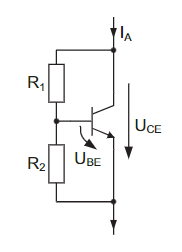
\includegraphics{tex/6_UBE-Vervielfacher/pictures/UBE_Schaltung.png}
    \caption{$U_{BE}$-Vervielfacher}
    \label{fig:my_label}
\end{figure}

\section{Berechnungen}

\subsection{Berechnung von $U_{CE}$ unter Vernachlässigung von $I_B$}

Der Strom $I_B$ teilt sich in 2 Teile auf: $I_R$ (der Strom durch die Widerstände) und den Kollektorstrom $I_C$ (der auch dem Emitterstrom entspricht). Eine einfache Masche zeigt, dass am Widerstand $R_2$ die Spannung $U_{BE}$ anliegt, somit ergibt sich der Strom durch die beiden Widerstände:

\begin{equation*}
    I_R \cdot R_2 = U_{BE} = \SI{0.7}{\volt} \rightarrow I_R = \frac{U_{BE}}{R_2}
\end{equation*}

Eine weitere Masche besagt, dass $U_{CE}$ die Spannung über die Widerstände $R_1$ und $R_2$ ist:

\begin{equation*}
    U_{CE} = I_R \left( R_1 + R_2 \right) = U_{BE} \frac{R_1 + R_2}{R_2} = U_{BE} \left( 1 + \frac{R_1}{R_2} \right) = \SI{0.7}{\volt} \left( 1 + \frac{R_1}{R_2} \right)
\end{equation*}

\newpage
\subsection{Berechnung von $U_{CE}$ unter Berücksichtigung von $I_B$}

Grundlegende Transistorgleichungen und Schaltungseigenschaften. 

\begin{align*}
    {} & I_{C} = I_S \left( e^{\frac{U_{BE}}{U_T}} - 1\right) & {}\\
    {} & I_{B} = \frac{I_C}{B} & {}\\
    K1: & I_A = I_{R_{1}} + I_C & {}\\
    K2: & I_{R_{1}} = I_{R_{2}} + I_B & {}\\
    K3: & I_A = I_{R_2} + I_C \left( 1 + \frac{1}{B} \right) & {}\\
    {} & I_A = I_{R_2} + I_B \left( 1 + B \right) &\rightarrow  I_B = \frac{I_A - \frac{U_{BE}}{R_2}}{B+1} \\
    {} & {} &  I_C = \frac{B \left(I_A - \frac{U_{BE}}{R_2}\right)}{B+1} \\
    M1: & I_{R_{2}} = \frac{U_{BE}}{R_{2}} & {}\\
\end{align*}

Wenn man $M1$ in $K2$ einsetzt erhält man:

\begin{equation*}
    I_{R_1} = \underbrace{\frac{U_{BE}}{R_{2}}}_{I_{R_2}} + \underbrace{\frac{I_S}{B} \left( e^{\frac{U_{BE}}{U_T}} - 1\right)}_{I_B = \frac{I_C}{B}}
\end{equation*}

Damit erhält man die gewünschte Funktion $U_{CE}\left( U_{BE}, I_A \right)$:

\begin{align}
    U_{CE}\left( U_B, I_A \right) &= U_{BE} + I_{R_1} R_1 = U_{BE} + R_1 \left( \frac{U_{BE}}{R{2}} + \frac{I_S}{B} \left( e^{\frac{U_{BE}}{U_T}} - 1\right) \right) \\
    &= U_{BE} \left( 1 + \frac{R_1}{R_2 }\right) + R_1 \frac{I_S}{B} \left( e^{\frac{U_{BE}}{U_T}} - 1\right)
\end{align}

In dieser Funktion kommt $I_A$ nicht vor, alternativ:

\begin{align}
    U_{CE}\left( U_B, I_A \right) &= U_{BE} + I_{R_1} R_1 = U_{BE} + \left( I_A - I_C \right) R_1 \\
    &= U_{BE} + \left( I_A - \frac{B \left(I_A - \frac{U_{BE}}{R_2}\right)}{B+1} \right) R_1 \label{UCE_glg}
\end{align}

\subsection{Bestimmung von $\frac{\Delta U_{CE}}{\Delta I_A}$}

Zur Bestimmung dieses Ausdrucks wird Gleichung \ref{UCE_glg} nach $I_A$ abgeleitet:

\begin{equation}
    \frac{\partial U_{CE}\left( U_B, I_A \right)}{\partial I_A} = 
    R_1 - R_1 \frac{B}{B+1} = R_1 \left( 1 - \frac{B}{B+1} \right) \label{dIA_simple}
\end{equation}

Bei hinreichend großer Verstärkung $B$ verschwindet diese Abhängigkeit.

\subsection{Bestimmung der $I_A$-Abhängigkeit aus dem Kleinsignalersatzschaltbild}

Um ein passendes Kleinsignalersatzschaltbild zeichnen zu können muss ein Ausdruck für $r_{BE}$ in Abhängigkeit von $U_{BE}$ und $I_{A}$ gefunden werden:

\begin{equation*}
    S \approx \frac{I_{C,0}}{U_T} = \frac{B \left(I_A - \frac{U_{BE}}{R_2}\right)}{U_T (B+1)}
    \quad 
    r_{BE} \approx \frac{B}{S} = \frac{U_T (B+1)}{I_A - \frac{U_{BE}}{R_2}}
\end{equation*}

Anschliessend können die Ströme im KSESB berechnet werden:

\begin{figure}[H]
    \centering
    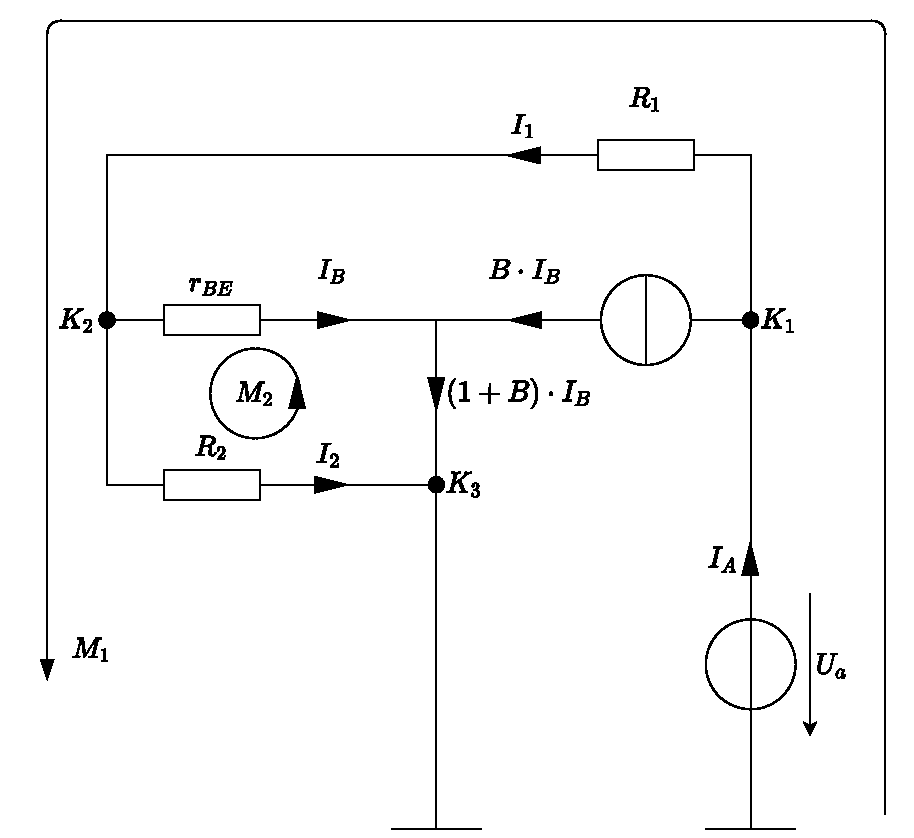
\includegraphics[width = 0.55\textwidth]{tex/6_UBE-Vervielfacher/pictures/KSESB.pdf}
    \caption{KSESB des $U_{BE}$-Vervielfachers}
\end{figure}

\begin{align*}
    K1:& I_A = B \cdot I_B + I_1 \\
    K2:& I_1 = I_B + I_2 \\
    K3:& I_A = I_2 + I_B (B+1)\\
    M1:& U_A = I_1 R_1 + R_2 I_2 \\
    M2:& R_2 I_2 = r_{BE} I_B \rightarrow I_B = \frac{R_2 I_2}{r_{BE}}
\end{align*}

$I_B$ aus $M2$ eingesetzt in $K3$:

\begin{align*}
    I_A = I_2 + \frac{R_2 I_2}{r_{BE}} (B+1) = I_2 \left( 1 + R_2\frac{B+1}{r_{BE}}\right) \rightarrow I_2 = \frac{I_A}{1 + R_2\frac{B+1}{r_{BE}}}
\end{align*}

$I_B$ aus $M2$ eingesetzt in $K2$:

\begin{align*}
    I_1 = \frac{R_2 I_2}{r_{BE}} + I_2 = I_2 \left( \frac{R_2}{r_{BE}} + 1 \right) \xrightarrow[]{I_2 \text{ eingesetzt}} I_1 = I_A \frac{\frac{R_2}{r_{BE}} + 1}{1 + R_2\frac{B+1}{r_{BE}}} \\
\end{align*}

Damit ergibt sich die Ausgangsspannung zu: 

\begin{align*}
    U_A =& R_1 I_1 + R_2 I_2 = R_1 \frac{I_A}{1 + R_2\frac{B+1}{r_{BE}}} + R_2 \frac{I_A}{1 + R_2\frac{B+1}{r_{BE}}} \left( \frac{R_2}{r_{BE}} + 1 \right)\\
    U_A =& \frac{I_A}{1 + R_2\frac{B+1}{r_{BE}}} \left( R_1 + R_2 \left( \frac{R_2}{r_{BE}} + 1 \right) \right)
\end{align*}

Bevor man nach $I_A$ ableitet muss noch $r_{BE}$ eingesetzt werden:

\begin{align*}
    U_A =& \frac{I_A}{1 + R_2
    \frac{I_A - \frac{U_{BE}}{R_2}}{U_T}
    } \left( R_1 + R_2 \left( \frac{R_2}{\frac{U_T (B+1)}{I_A - \frac{U_{BE}}{R_2}}} + 1 \right) \right)
\end{align*}

Nach Einsatz von Computeralgebra (Sympy) folgt: 

\begin{align}
    \frac{\partial U_A (I_A)}{\partial I_A} =& \frac{I_{A} R_{2}^{2}}{\left(B + 1\right) \left(I_{A} R_{2} + U_{T} - U_{BE}\right)} - \frac{I_{A} R_{2} \left(R_{1} U_{T} \left(B + 1\right) + R_{2} \left(I_{A} R_{2} + U_{T} \left(B + 1\right) - U_{BE}\right)\right)}{\left(B + 1\right) \left(I_{A} R_{2} + U_{T} - U_{BE}\right)^{2}} \nonumber\\ &+ \frac{R_{1} U_{T} \left(B + 1\right) + R_{2} \left(I_{A} R_{2} + U_{T} \left(B + 1\right) - U_{BE}\right)}{\left(B + 1\right) \left(I_{A} R_{2} + U_{T} - U_{BE}\right)} \label{dIA_complex}
\end{align}

Dieser Ausdruck ist wesentlich komplexer als jener aus Gleichung \ref{dIA_simple}. Dies ist zurückzuführen auf ???

\subsection{Verwendung des 2k2-Potentiometers}

Im letzten Unterpunkt dieser Aufgabe soll die Schaltung so dimensioniert werden, so dass ein Widerstand durch das 2k2-Potentiometer ersetzt wird und sich die Kollektoremitterspannung über veränderungen der Potentiometerstellung von $U_{BE}$ bis $\SI{3}{\volt}=4.286 \cdot U_{BE}$ einstellen lässt. Dazu sollte die einfache Formel aus dem ersten Unterpunkt verwendet werden:

\begin{equation*}
     U_{CE} = U_{BE} \left( 1 + \frac{R_1}{R_2} \right)
\end{equation*}

Es ist offensichtlich, dass das Verhältniss $R_1$ zu $R_2$ im Intervall $0 \ldots 3.286$ variiert werden muss. Der Widerstand $R_1$ wird durch das Potentiometer ersetzt. Wenn $R_1$ seinen maximalwert von \SI{2.2}{\kilo \ohm} erreicht, muss gelten:

\begin{equation*}
    \frac{R_1}{R_2} = \frac{\SI{2.2}{\kilo \ohm}}{R_2} = 3.286 \rightarrow R_2 = \frac{\SI{2.2}{\kilo \ohm}}{3.286} = \SI{513}{\ohm}
\end{equation*}

Mit einem \SI{510}{\ohm} Widerstand aus der E24-Reihe wäre man also gut beraten.
